% \begin{frame}
%     \frametitle{Lemma 1 - Brodcast Conformity}
%     \begin{lemma}
%         If a correct process $p_i$ recives a message $m$ from a $r\_brodcast(m)$ by another correct process - 
%         any other correct process will recive $m$.\\
%     \end{lemma}

%     \begin{proof}
%         Immidiate from the guarantees of the broadcast algorithm.
%     \end{proof}
% \end{frame}
\begin{frame}
    \frametitle{Correct Process Intersection}
    \begin{lemma}
        Any two sets of processes of size $(n-t)$ must have
        at least one correct process in common.
    \end{lemma}
    \begin{center}
        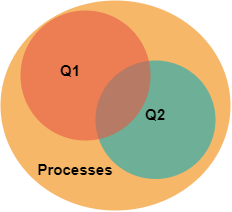
\includegraphics[scale=.5]{resources/lemma2_venn.png}
    \end{center}
\end{frame}
\begin{frame}
    \frametitle{Correct Process Intersection. Proof.}
    \begin{proof}
        Denote the set of processes with $P$, and the set of faulty ones $F$.\\
        Let $Q_1,Q_2\subseteq P$ s.t. $|Q_1|=|Q_2|=n-t$.\\
        \[
            |\overline{Q}_1\cup\overline{Q}_2|\leq |\overline{Q}_1|+|\overline{Q}_2|
            \Rightarrow n-|\overline{Q}_1\cup\overline{Q}_2|\geq n-|\overline{Q}_1|-|\overline{Q}_2|
        \]\[
            \Rightarrow |\overline{\overline{Q}_1\cup\overline{Q}_2}|\geq n-t-t
        \]\[
            \Rightarrow |Q_1\cap Q_2|\geq n-2t>3t-2t=t=|F|
        \]\[
            \Rightarrow \exists p\in Q_1\cap Q_2\notin F
        \]
    \end{proof}
\end{frame}

\subsection{Termination Properties}
\begin{frame}
    \frametitle{Write Termination}
    \begin{lemma}
        Let $p_i$ be a correct process.
        Any invocation of $Reg[i].write()$ terminates.
    \end{lemma}
    \begin{proof}
        By induction; Assume $k$'th write invocation by $p_i$ recives $WRTIE\_DONE$ from $n-t$ correct processes.
        \begin{itemize}
            \item When $p_i$ invokes write for $k+1$ time, it brodcasts $WRITE$.
            \item $n-t$ correct processes recive $WRITE$ (eventually).
            \item In each of those, $reg[j].sn$ is $k$ due to induction assumption (line 12).
            \item (line 12) satisfied and $WRITE\_DONE$ is sent back.
        \end{itemize}
    \end{proof}
\end{frame}
\begin{frame}
    \frametitle{Read Termination}
    \begin{lemma}
        Let $p_i$ be a correct process. Any invocation of $Reg_i[j].read()$ terminates.
    \end{lemma}
\end{frame}
\setbeamertemplate{itemize items}[circle]
\begin{frame}{Read Termination. Proof.}
    \begin{block}{(*) Conclusion from Write Termination lemma}
        If one correct process get's to $Reg[j].sn=k$ ($p_j$ is also correct),
        then all correct processes eventually have $Reg[j].sn\geq k$.\\
        Otherwise - they could not send $WRITE\_DONE$ to
        $p_j$ in contrediction to write termination.
    \end{block}
    Assume $read[i,j,\cdot]$ - meaing $p_i$ invokes $Reg[j].read()$.
    \begin{block}{Line (7) termination}
        \begin{itemize}
            \item Denote $m$ as the max (min-max...) index recived at line (7).
            \item This means some correct process $p_k$ must have $Reg[j].sn=m$.
            \item Due to (*), $p_i$ eventually gets $Reg[j].sn=m$ too.
        \end{itemize}
    \end{block}
    % Druring the read, $p_i$ brodcasts $READ(j,rsn)$ where $rsn$ is a sequence number 
    % unique to this read. Due to reliable brodcast, $n-t$ correct processes recive and handle
    % it eventually and sends a value $wsn_k$. Now cosider that $p_k$ (a correct process)
    % has sent $wsn_k=Reg_k[j].sn$, meaning at some point it must have recived a
    % reliable brodcast message $WRITE(\_,wsn_k)$, due to lemma 1 - this means $p_i$ will
    % eventually recive $WRITE(\_,wsn_k)$ too. At that point, $Reg_i[j].sn$ will also
    % be at-least $wsn_k$.\\
    % So eventually - there are $n-t$ correct processes sending $STATE(\_, wsn_k)$
    % and for each $Reg_i[j]\geq wsn_k$ eventually. This means line (7) will finish at some point.\\
\end{frame}
\begin{frame}{Read Termination. Proof.}
    \begin{block}{Line (10) termination}
        \begin{itemize}
            \item $p_i$ sends $wsn:=Reg[j].sn$.
            \item All correct processes recive $CATCH\_UP(j,wsn)$.
            \item Due to (*), each one eventually has $Reg[j].sn = wsn$, meaning they finish wait at (16).
            \item So each one sends back $CATCH\_UP\_DONE$.
        \end{itemize}
    \end{block}
    % The next possible stall to the \emph{read} invocation is at line (10) -
    % \emph{'wait $CATCH\_UP\_DONE(j,x)$' from $n-t$ different processes}.\\
    % At line (9) we brodcast $CATCH\_UP(j,x)$, so all correct processes
    % eventually recive it. Consider $p_k$ which has recived $CATCH\_UP(j,x)$;
    % for $p_i$ to have arrived when $Reg_i[j].sn=x$, all $WRITE$ messages 
    % of the first $x$ writes by $p_j$ must have arrived at $p_i$, due to reliable
    % brodcast - all these messages must arrive at $p_k$ too. When the last of them does - 
    % $Reg_k[j].sn$ is at-least $x$ causing the wait at line (16) to terminate thus
    % $p_k$ sends $CATCH\_UP\_DONE(j,x)$ to $p_i$.\\
    % When the last process $p_k$ sends $CATCH\_UP\_DONE$ - $p_i$ can terminate.
\end{frame}

\subsection{Atomicity Properties}
\begin{frame}
    \frametitle{Write Serialization}
    \begin{lemma}
        It is possible to associate a single sequence of values $H_i$
        with each register $Reg[i]$. Moreover, if $p_i$ is correct -
        $H_i$ is the sequence of values written to $Reg[i]$ by $p_i$.
    \end{lemma}
\end{frame}
\begin{frame}
    \frametitle{Read before Write}
    \begin{lemma}
        Let $p_i, p_j$ be two correct processes.\\
        If $read[i,j,x]$ terminates before $write[j,y]$ starts, then $x<y$.
    \end{lemma}
\end{frame}
\begin{frame}
    \frametitle{Read before Write. Proof.}
        %write: wait for everyone to be at your serial number then finish writing.

        %read: wait for your serial number to be at least that of n-t others at the time
        % or read starts. then wait for n-t others to get to that last serial number.
        Assume $read[r,w,sn_r]$ before $write[w,sn_w]$, meaning $p_r$ read $Reg[w]$
        before $p_w$ wrote to it.
        \begin{itemize}
            \item Denote $Q_r$ the processes which terminated line (10).
            \item Denote $Q_w$ the processes which terminated line (3).
            \item Thanks to correct process intersection lemma: $\exists p_k\in Q_1\cap Q_2$.
            \item Denote $p_k$'s serial number when $CATCH\_UP\_DONE$ was sent with $sn_k$. 
            \item Due to line (16), $sn_r\leq sn_k$.
            \item Denote $sn_k'$ the serial number at $p_k$'s when wait at (12) finshed.
            \item Due to line (12), $sn_w=sn_k'+1$.
            \item $sn_r\leq sn_k\leq sn_k'= sn_w-1\Rightarrow sn_r < sn_w$.
        \end{itemize}
\end{frame}
\begin{frame}
    \frametitle{Write before Read}
    \begin{lemma}
        Let $p_i, p_j$ be two correct processes.\\
        If $write[i,x]$ terminates before $read[j,i,y]$ starts, then $x\leq y$.
    \end{lemma}
\end{frame}
\begin{frame}
    \frametitle{Write before Read. Proof.}
    Assume $write[w,sn_w]$ before $read[w,r,sn_r]$, meaning $p_w$ wrote 
    before $p_r$ read from $Reg[w]$.
    \begin{itemize}
        \item Denote $Q_w$ the processes which terminated line (3).
        \item Denote $Q_r$ the processes which terminated line (7).
        \item $\exists p_k\in Q_1\cap Q_2$.
        \item Denote $sn_k$ the serial number at $p_k$'s when wait at (12) finshed.
        \item Due to line (12), $sn_w=sn_k+1$.
        \item Denote $p_k$ serial number when $STATE$ was sent with $sn_k'$.
        \item Due to line (7), $sn_r\geq sn_k'$.
        \item $sn_w=sn_k+1\leq sn_k'\leq sn_r\Rightarrow sn_w\leq sn_r$.
    \end{itemize}
\end{frame}
\begin{frame}
    \frametitle{No Read Inversion}
    \begin{lemma}
        Let $p_i, p_j$ be two correct processes.\\
        If $read[i,k,x]$ terminates before $read[j,k,y]$ starts, then $x\leq y$.
    \end{lemma}
\end{frame}
\begin{frame}
    \frametitle{No Read Inversion. Proof.}
    Assume $read[r_1,j,sn_1]$ before $read[r_2,j,sn_2]$, meaning $p_1$ read
    before $p_2$ from $Reg[j]$.
    \begin{itemize}
        \item Denote $Q_1$ the processes which terminated line (10) in $p_1$'s run.
        \item Denote $Q_2$ the processes which terminated line (7) in $p_2$'s run.
        \item $\exists p_k\in Q_1\cup Q_2$.
        \item Denote $sn_k$ the serial number at $p_k$ when wait at (16) finished.
        \item Due to line (16), $sn_k\geq sn_1$.
        \item Denote $sn_k$' the serial number sent from $p_k$ to $p_2$ as $STATE$.
        \item Due to line (7), $sn_k'\leq sn_2$.
        \item $sn_1\leq sn_k\leq sn_k'\leq sn_2$.
    \end{itemize}
\end{frame}

\subsection{Piecing it all together}
\begin{frame}
    \begin{theorem}
        The algorithm showcased implements and array of $n$ SWMR
        registers with atomic Consistency, in $BAMP$ with $t<\frac{n}{3}$ systems.
    \end{theorem}
    \begin{proof}
        We have seen required termination properties in lemmas 3,4 and atomicity
        properties in lemmas 5,6,7,8.\\
    \end{proof}
\end{frame}

\begin{frame}
    \frametitle{Complexity}
    
    \begin{block}{Read Complexity}
        \alert{$O(n)$} messages are required for each read - as can be seen
        by the brodcasts at lines (6) and (9).
    \end{block}
    \begin{block}{Write Complexity}
        \alert{$O(n^2)$} messages are required for each write,
        since for a \alert{reliable} brodcast is required
        by the write invocation - which could require up to $O(n^2)$
        messages to be sent. 
    \end{block}
\end{frame}